\chapter{Distributing software artifacts in IoT systems}
\label{ch:softArtDist}
%We discussed in the previous chapters how the IoT will have a huge impact in our everyday activities.
%As a result, the presence of IoT devices in our environment will form a typical distributed system, on which we aim to deploy applications and maintain them in an updated state, as well as stop or remove them if desired.
%Some challenges raised by this dynamic behavior were already exposed in the previous chapter, concluding by the proposal of a model@runtime as an abstraction and management approach for the software layer.
%As illustrated previously, managing evolution of this software layer is a major issue.
%In the software engineering community, software reconfiguration are realized through various techniques such as: service oriented computing \cite{papazoglou2003service}, component oriented computing \cite{szyperski1999component} or models@runtime \cite{morin2009}  to achieve behavior evolution of a distributed system.
Throughout this thesis, we have noticed three important characteristics of IoT systems: (1) they are distributed, (2) they include resource constrained nodes especially in memory and energy, (3) they are heterogeneous both in hardware infrastructure and role in the network. 
Indeed, the heterogeneity is an important factor as it encompasses the hardware and software layer: each node composing the network has its own role in it, and thus its specific hardware and software configurations which will evolve over time.
As we presented in the introduction of chapter \ref{ch:MARContiki}, solutions from the domain of Software Engineering can deal with this problem, but cannot be seamlessly adapted to fit with all the characteristics of an IoT system, especially with the resource constrained nodes.
Therefore, a first approach is to propose a way to decompose this systems into components, leveraging the benefits argued by CBSE. This was already discussed in the previous chapters, showing that a model@runtime can represent this decomposition in the model.
However, decompose this software in components raise the question about their distribution in a typical IoT network.

As a consequence, in this chapter we will address the following scientific problem: \textbf{How to \textit{efficiently} distribute, deploy and configure software components for IoT devices?}

Following our initial experiments presented in the chapter \ref{ch:MARContiki}, our M@R implementation provides an abstraction layer (which is simpler and safer to manipulate than the actual system) to tame the complexity of software adaptation in a distributed system. 
The software layer is represented as a set of interconnected components which are then deployed and configured on each node.
Following this approach, deploying and reconfiguring software requires distributing the code of the specific software components to the targeted nodes.
Currently, state of the art approaches to disseminate code over the air are limited in their ability to select specific targets (they disseminate the same binary to every node in the network\cite{hui2004dynamic}), and thus waste energy when all nodes do not present an homogeneous software layer.
Another approach called FiGaRo\cite{mottola2008figaro} propose the use of rules to filter nodes regarding its use or current capacities, in order to select some of them for an update or new deployment, thus a fine selection of an specific node becomes complicated.

In this chapter, we present an extension on the use of models@runtime to represent both the network and the application layer of the Internet of Things systems.
At runtime, we leverage these models through a new algorithm to distribute a software component only to those devices that need it, providing a fine selection by manipulating the model directly.
Moreover, this new algorithm aims at minimizing energy consumption during the whole reconfiguration and adaptation step, proposing a distribution mechanism which performs this task in a very efficient manner.

After an overview of our current approaches,  we explain how the minimalistic Kevoree component model was implemented, followed by the main challenges while distributing the actual components in a binary form.
Afterwards, a study of the possible distribution mechanisms is done, concluding with the proposition of a new algorithm for components distribution.
Finally, our representative experiments are conducted on the FIT-IoT Lab testbed, in order to evaluate the algorithms and show our results regarding energy consumption and time to deploy such components.

\section{Overview}
We have evaluated our algorithms on a representative scenario taken from a real deployment scenario.
Indeed, our algorithm was implemented in the IoT-Lab testbed \cite{Fleury15iotlab} with a specific configuration of 10 nodes, as a starting point.
While the availability of a huge number of nodes in a testbed seems to be adequate for a large deployment experiment, some difficulties were encountered during experimentation, regarding the network topology and routing protocols restrictions.
This is due to the layout of the physical deployment on the testbed, since the nodes are too close to each other, making difficult to build a mesh with several hops.
Therefore, modifications to the transmission power and sensibility of the radio interfaces have been done, in order to have a good topology to run the tests.
As for the routing protocols, we used ContikiRPL\cite{tsiftes2010contikirpl}, an implementation of the RPL\cite{rfc6550} protocol for LLNs and 6loWPAN.
This protocol triggers regularly a "rebuilding" of the topology, thus parents and childs can change even if the nodes do not move.
Indeed, this modification can change the behavior of our algorithm, thus our experiments must be run several times using the same configurations.
Even so, the representative results on 10 nodes show that our approach performs better regarding energy efficiency and deployment time in comparison to state of the art algorithms.
%This leaded our experimentations to a large set of nodes using the Cooja\cite{osterlind2006cross} simulator, in order to have a more controlled network topology which allows to compare the performance of our protocol.

We can summarize the contributions of this chapter as follows:
\begin{itemize}
	\item \textbf{Leverage the already described modeling tools to configure and re-configure IoT systems.} This approach provides a view of a running Internet of Things system on its current state and an efficient way of reconfiguring the software layer of these systems.
	\item \textbf{An energy efficient algorithm to disseminate software components.} This algorithm leverages the network topology and the information contained in the model to decide locally on the best way to disseminate software components.
	\item \textbf{An evaluation of the algorithm on a network of real sensor nodes.} The main experiment aims at evaluating the energy consumption of software reconfigurations using our approach on a network of real sensors using the IoT-lab platform.
\end{itemize}


The next section will present our proposition to divide an IoT application into components, following the component model proposed on the kevoree meta-model.
%Throughout this chapter, which are followed by the extensive simulation on Cooja showing the scalability of our approach.

%\section{Overview}

\section{Componentization of applications in the IoT}
One of the main challenges discussed on this chapter consists in decomposing IoT applications into smaller pieces in order to ease development and maintenance.
Several approaches have already proposed component models for embedded systems\cite{friedrich2001survey} and WSN \cite{marron2006flexcup}, \cite{grace2004gridkit}, \cite{mottola2008figaro}, \cite{cid2012looci}, \cite{taherkordi2013optimizing}, on which the concepts already discussed in \ref{sec:CBSE} are leveraged to bring reconfiguration facilities onto this architectures.
Indeed, many similarities can be found between embedded systems, WSN and the IoT, mostly on the resource constrained nodes being part of these networks.
However, the network size, used protocols and applications complexity in IoT systems demand a different approach.

Our proposition based on a Model@runtime\cite{morin2009mar} presented in section \ref{sec:MAR_overview}, a paradigm which aims at simplifying the development of distributed dynamically adaptable systems, proposes the use of a model which represents the system state as depicted in Figure \ref{fig:MAROverview2}. 
This model can then be synchronized with the real running system: 
\begin{itemize}
	\item any change in the system state is reflected into the model,
	\item any change in the model will be sent to the running system which will adapt its behavior to reflect these changes. 
\end{itemize}
These two way synchronization can be done automatically or on demand.

Model@runtime is generally used together with a component based software architecture.
In component based software architecture, an application is broken into different software pieces called software components which are linked together through software connectors \cite{dashofy2002infrastructure,medvidovic2000classification,van2000koala} to from the architecture of the application.
Software components can then be deployed independently at remote locations as illustrated in Figure \ref{fig:MAROverview2}. 
One of the benefits is that it facilitates the management of dynamic applications, which is a primary concern for IoT systems deployed in constantly evolving environments.

\begin{figure}[htb]
	\centering
	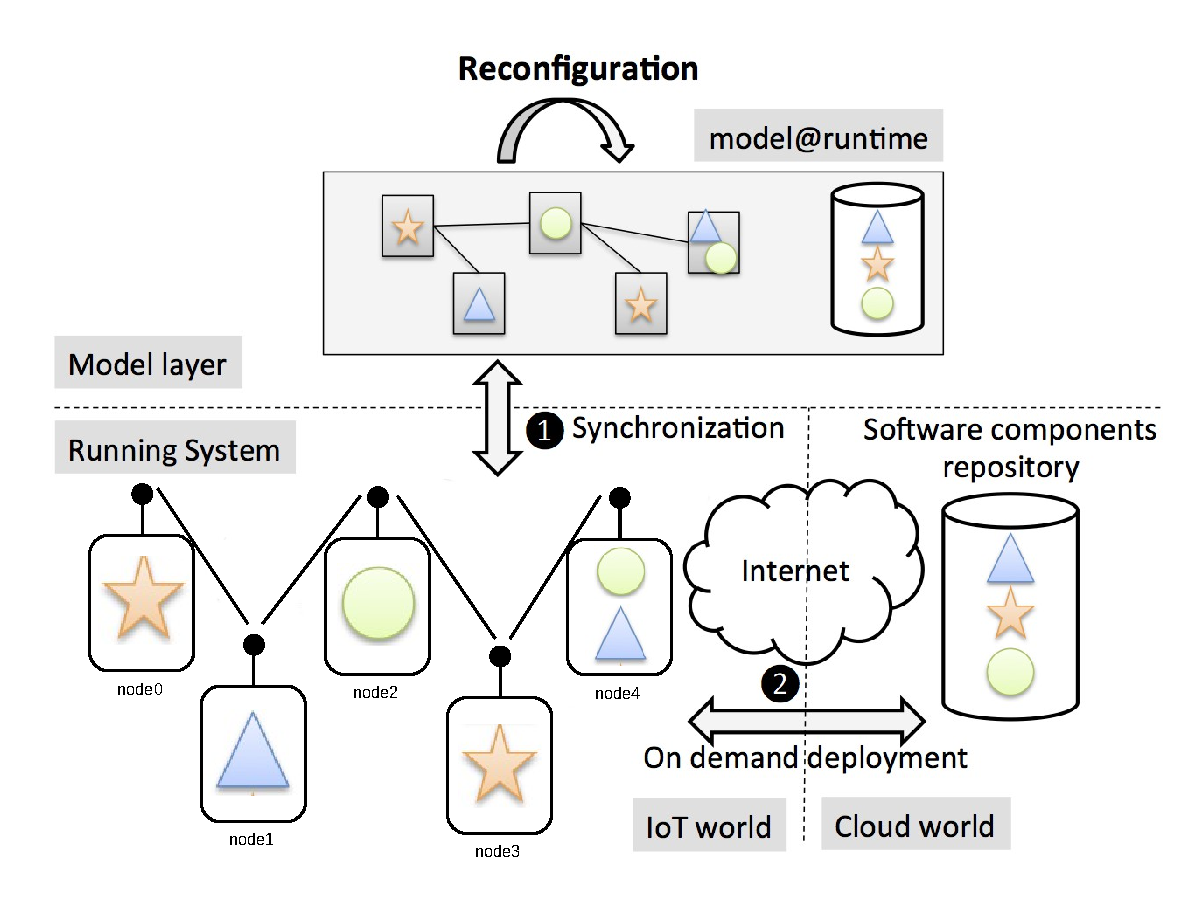
\includegraphics[width=0.95\columnwidth]{chapters/calpulli.images/MAR_Overview2.pdf}
	\caption{Model@runtime principle} \label{fig:MAROverview2}
\end{figure}

When using component based software architecture together with the model@runtime paradigm, the model layer represents the software architecture (a set of software components and connectors) mapped onto the distributed physical execution environment.
Any change made in the software architecture triggers an adaptation on the real system in order to deploy, remove or update software components or connectors.   

\begin{figure}[htb]
	\centering
	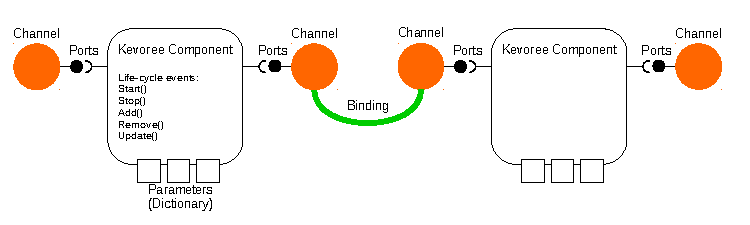
\includegraphics[width=0.95\columnwidth]{chapters/calpulli.images/componentModel.pdf}
	\caption{Kevoree component model} \label{fig:kevCompModel}
\end{figure}

Our component model can be represented as depicted in figure \ref{fig:kevCompModel}, on which the properties of a component are separated as follows:
\begin{itemize}
	\item \textit{Kevoree Component.} The instance itself containing the life-cycle events triggered either by an external event (through the Kevoree-IoT core) or by an internal adaptation (which will modify the model).
	\item \textit{Properties.} Internal properties or parameters are the configurable settings that modify the component's behavior.
	This properties are represented by a dictionary, which can be affected by an \textit{update} event.
	\item \textit{Ports.} In contrast with other component models, an extra abstraction for component's interaction is provided by our model.
	It consists in exposing the ports (interfaces) only to another instance called \textit{channel}, on which communication means are implemented in a separated way.
	\item \textit{Channel.} An independent instance which is very useful to avoid direct function calls between components.
	Indeed, instead of using direct function calls, a communication channel can apply different and more complex semantics, a valuable feature in distributed environments\cite{fouquet2013kevoree, barais2005construire}.
	\item \textit{Binding.} Is the representation of the connections between channels. Several bindings can exist per channel, in a point-to-multipoint schema.
\end{itemize}

\begin{figure}[htb]
	\centering
	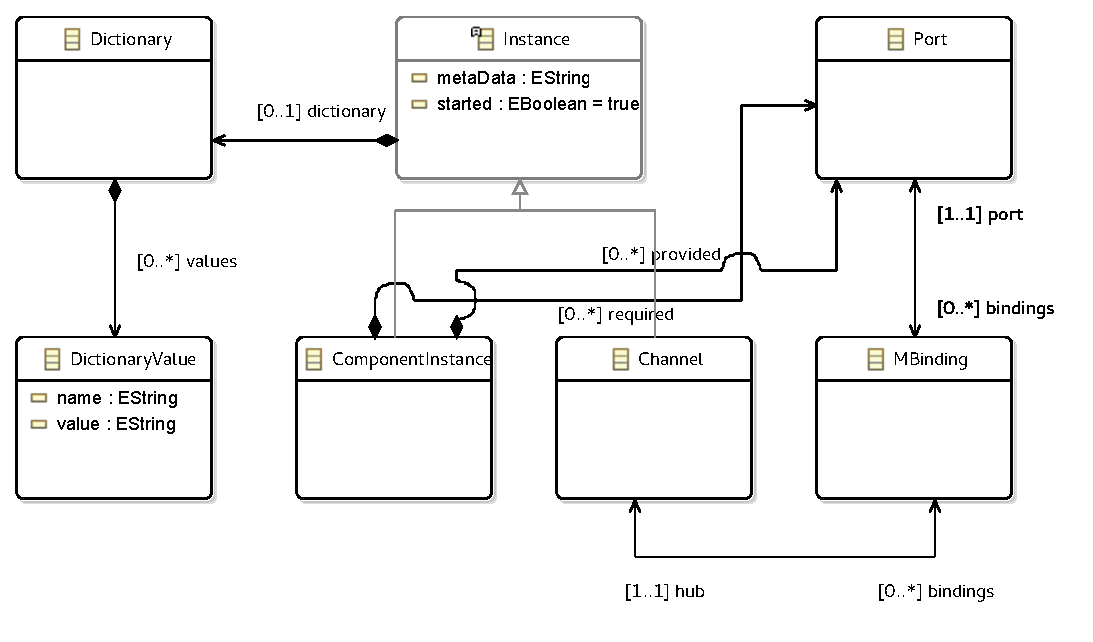
\includegraphics[width=0.95\columnwidth]{chapters/calpulli.images/ComponentModelUML.pdf}
	\caption{Component model from the Kevoree meta-model} \label{fig:kevCompModelUML}
\end{figure}

As for the Kevoree meta-model representation, we can observe in figure \ref{fig:kevCompModelUML} that a component instance can use an unlimited number of ports which can also have an unlimited number of bindings.
We can clearly identify a channel as a separated instance, thus the implementation is completely independent from the component.
Moreover, the dictionary abstraction allows to configure both channels and components, adding flexibility to the communication means.

\subsection{A component-based implementation for Contiki}
\label{subsec:contikiCompModel}
The implementation of this component based model was done by mapping the abstract concepts into data structures, as a part of a Contiki loadable module.
We leverage the Contiki's dynamic loader and linker feature described in \cite{dunkels06runtime}, as a method to load dynamically the components and create its instances.
Indeed, a Contiki process is used to register new components to the Kevoree-IoT core, which are then available in the form of deploy units.
Afterwards, once the loading is completed, we can affect the life-cycle of the application by creating new instances of the newly downloaded type.
Instance creation is done using a simple memory block allocation scheme, allowing to create as many instances as free memory is available.

This adaptation of the component model, even if it is very oriented to its use in a Contiki environment, was optimized to achieve a behavior very similar to the original Kevoree implementation, which is very high resource consuming.
Indeed, this task was very challenging due to the constrained resources of the nodes on which we aim to run our experiments.
Moreover, a more challenging problem raised while we tried to distribute components across the network.
While using a straightforward technique to reach the target node of a component, which consisted in a direct deploy unit download from a remote repository, we realized that this method was very energy consuming.
Indeed, every time a component was needed a considerable quantity of nodes in the mesh network were used to transport the packets to its final destination, and this was repeated for each node.
Thus, the new challenge lies in the way a component is disseminated on the network.
Indeed, providing the best path to download it and using local "cache" repositories to distribute a common component for several nodes could reduce energy consumption.
Therefore, a new distribution algorithm is needed in order to provide such functionality.
This new issues are discussed in the next Subsection.

\subsection{Challenges distributing software components in the IoT}
When changes in the model are disseminated in the IoT system, each node will adapt its local state to the new requirements. 
Indeed, this adaptation can include the deployment of one or several new components, as depicted in Figure \ref{fig:MAROverview2}. 
Moreover, a given component is not necessarily needed by all nodes in the network. 
Is in this part where state of the art algorithms to disseminate code over multihop WSNs are limited, since their ability to target specific nodes is poor or inexistent. 
For instance, the Deluge protocol\cite{hui2004dynamic} disseminates the same "data pages" of a whole firmware to every node, thus there is no fine selection of the nodes we want to upgrade. 
In order to deal with this limitation, we propose a new algorithm called \emph{Calpulli}, to efficiently perform the wireless distribution of components to the destination nodes. 
We leverage \textit{(a)} the routing properties of the running system and \textit{(b)} the information provided by the model to find the best strategy of components downloading.
Details of this protocol are discussed in the next section.

%\section{Requirements for artifacts distribution}
\section{Calpulli: A distributed algorithm for component dissemination}
Thanks to the available information, both the execution state of the system and routing details of the mesh network, it is possible to use both in order to provide a better component distribution to the targeted nodes.
This two features are described as following:

\paragraph{Routing properties of the running system.} Networks used by IoT systems are often referred to as Low power and Lossy Networks (LLNs). The \emph{Ripple} Routing Protocol (RPL)\cite{rfc6550} is a IPv6 routing protocol for LLNs that builds a Destination Oriented Directed Acyclic Graph (DODAG). This graph starts at the root/BR (Border Router), a specific node chosen by the system administrator and connected to the rest of the network. Each node in the graph has a rank that represents the number of hops to the root. In this hierarchy each node on the graph has a routing entry towards its parent and it can send a data packet to the BR by forwarding it to its immediate parent. Figure \ref{fig:MARdodag} gives an example of a simple DODAG within a 9-nodes network.

\begin{figure}[htb]
	\centering
	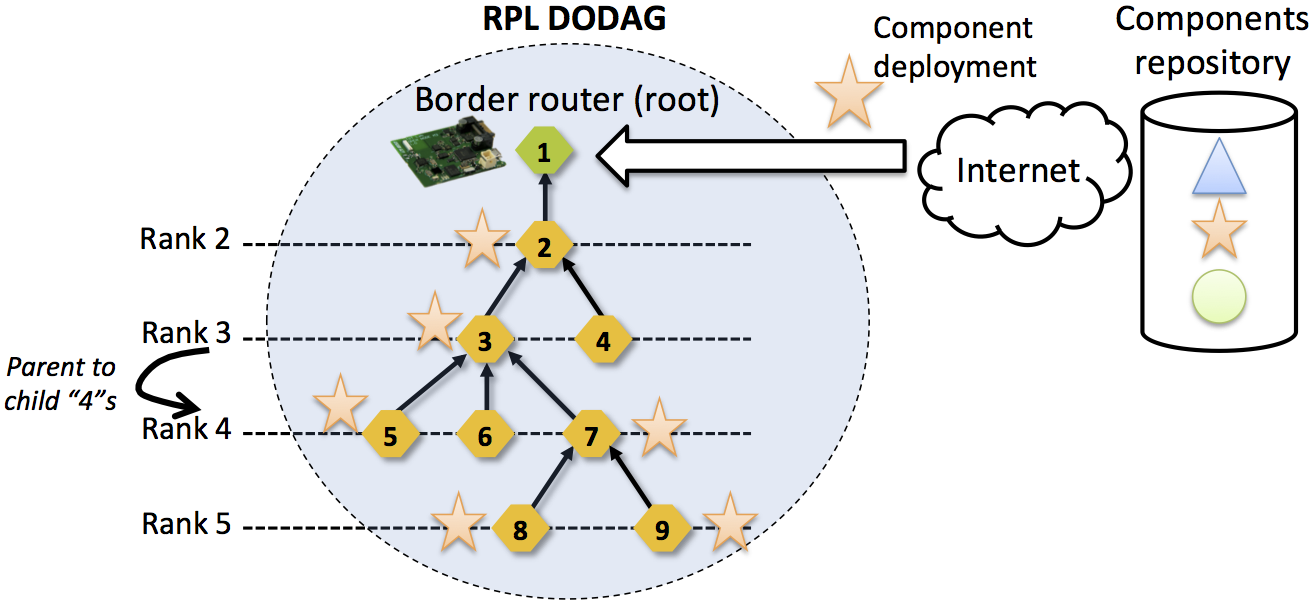
\includegraphics[width=0.98\columnwidth]{chapters/calpulli.images/MAR_dodag.png}
	\caption{Dissemination of software components using a DODAG} \label{fig:MARdodag}
\end{figure}

\paragraph{Information provided by the model@runtime} After a model synchronization, a node knows which components must be downloaded from the remote repository for its own adaptation.
Afterwards, a node is able to identify all the other nodes that request the same component by looking into the entire model.
In the example shown on Figure \ref{fig:MARdodag}, the component represented by the $\bigstar$ is needed by nodes identified as 2-3-5-7-8-9. 
Thanks to the model information, node 9 knows that the component $\bigstar$ is requested by nodes 2-3-5-7-8.

The objective of \emph{Calpulli} can be summarized as follows:
\begin{itemize}
	\item Among a set of nodes that targets the same component ($\bigstar$ in Figure \ref{fig:MARdodag}), \emph{Calpulli} chooses the nearest node from the BR (node 2).
	\item This "selected" node (called the \emph{repository node}) downloads the component and acts as a local repository for other nodes (nodes 3-5-7-8-9 in).
	\item All the other nodes wait for the repository node until it is ready to share the component $\bigstar$.
\end{itemize}

The selection process of the repository node for the component $\bigstar$ uses the hierarchical structure of the DODAG. When a node needs the component $\bigstar$, two cases can be considered:

\begin{enumerate}
	\item If the node knows that its parent in the DODAG targets the same component $\bigstar$, it has nothing to do. Its parent, with a lower rank, can be candidate to be the repository node and will immediately  download of the component.
	\item Otherwise the node can potentially play the role of the repository node for the component $\bigstar$. It sends to its parent a message containing its own address (to declare itself as the repository node) and a reference to the targeted component $\bigstar$.
\end{enumerate}

If a node receives a message from a child node asking for an unneeded component, it just forwards the message to its immediate parent without modification. The process is stopped when the BR is reached with a message containing the address of the "nearest node" that needs the component $\bigstar$.

%Details about the use of Calpulli to download new artifacts are given in the next Subsection.

%\subsection{Downloading artifacts using Calpulli}
The implementation of \textit{Calpulli} was integrated as a part of the Kevoree-IoT runtime, which leverages the available UDP sockets on Contiki to transport a component from a remote repository located on the Internet.
Indeed, a small protocol was developed to support \textit{Calpulli}, in order to establish synchronization between nodes acting either as \textit{"repositories} or \textit{"clients"}.
This protocol aim to use the repository address determined by \textit{Calpulli}, and to transform any node into a repository.

\begin{figure}[]
	\centering
	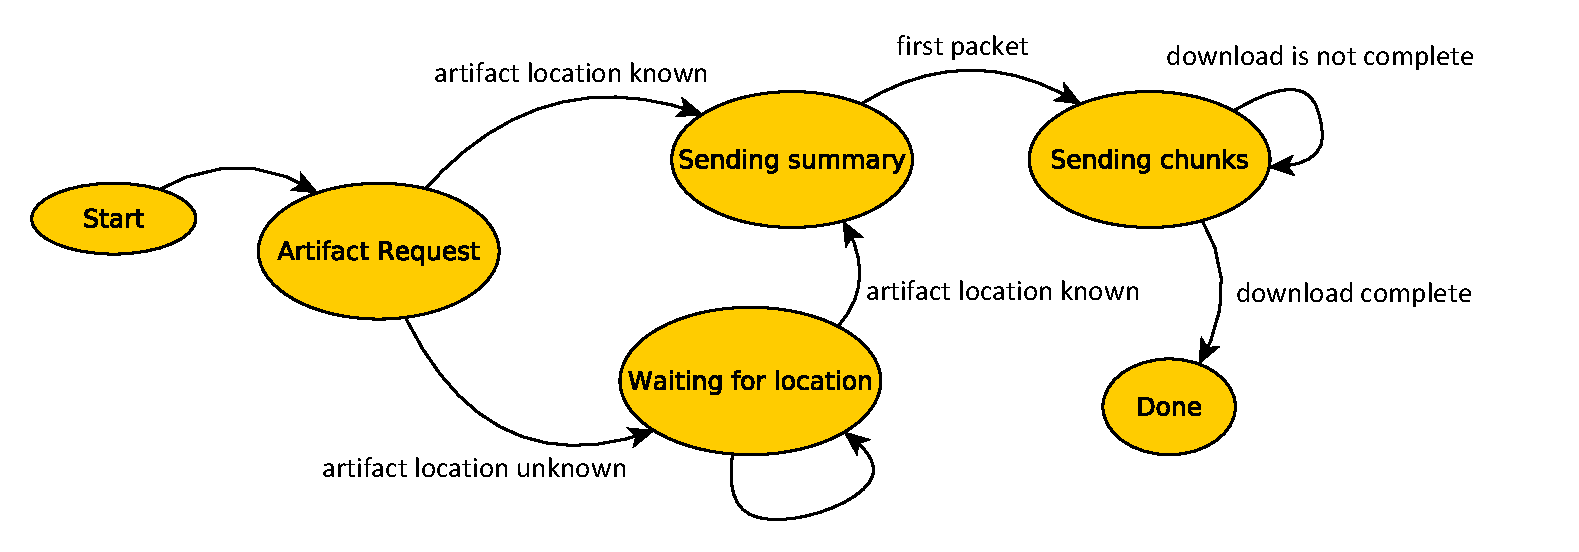
\includegraphics[width=0.98\columnwidth]{chapters/calpulli.images/calpulliProtocol.pdf}
	\caption{State diagram describing a new artifact download, acting as a repository} \label{fig:calpulliProtocol}
\end{figure}

In Figure \ref{fig:calpulliProtocol}, a state-transition diagram is used to represent the proposed protocol for artifacts downloading.
As we can observe, once \textit{Calpulli} has determined the nearest repository candidate, an artifact request is sent to such node which will first determine if the artifact location is known (if the requested deploy unit was already downloaded). Afterwards, if the location is unknown, it will ask directly to the main repository (a central repository outside the local network).
When the location is known (deploy unit downloaded), a summary is sent to the \textit{"client"}, indicating details about the size and number of chunks that will be sent.
Afterwards, the server will receive a response asking for the chunks composing the deploy unit.
When the download is over the node stops the protocol and will look for the next request, if any.

In order to evaluate \textit{Calpulli}, a series of experiments should be carried on.
The goal is to assess the energy savings provided by the algorithm, in comparison with state of the art algorithms for firmware updates, as well as the time needed to perform such update.

%\subsection{First approach: Kevoree algorithm}

%\subsection{Particularities of a typical IoT network topology}

\section{Evaluation}
In this section, we evaluate the performance of the \textit{Calpulli} algorithm with respect to energy consumption and delay to distribute software components.
The energy consumption is related to the amount of transmissions on all nodes in the mesh network, since a data packet can be retransmitted by several nodes before reaching its destination.
The time to deploy covers the delay between an artifact request and the deployment of the requested component.

\subsection{Use case}
In our scenario, 10 selected nodes on the IoT-Lab testbed are preloaded with a firmware containing \textit{Kevoree-IoT}, \textit{Calpulli} and a UDP client/server which will act as a components repository when needed.
Moreover, a set of components were available on a central repository running on a PC, which was interfaced with the testbed through a SSH tunnel to a border router. This PC is representing the main repository available on Internet, thus external to the IoT network.

Our goal for this use case is to answer the following research questions: 
\paragraph{RQ1}: Does \textit{Calpulli}, our dedicated software components distribution algorithm, consumes less energy in average than state of the art algorithms for firmware/components distribution?

\paragraph{RQ2}: Is \textit{Calpulli} quicker to distribute software components than state of the art algorithms?

\subsection{Experimental setup}
This evaluation is based on experiments done with a set of physical nodes presented in the previous Subsection.
All the experiments described in this section have been carried out on the IoT-Lab testbed\cite{Fleury15iotlab}.
% already described in \ref{sec:iotlab}.
%IoT-Lab is a platform that aims to provide a full IoT environment, from very small nodes (based on msp430 MCU) to very big nodes (based on Cortex-A9 CPU), including a "middle" sized node (based on Cortex-M3 MCU).
Indeed, our experiments are designed to fit a "class 2" sized node, which is called "iot-lab M3" on this platform.
The choice of this node is done based on precedent analysis of performance in different nodes \cite{tsekoura2014evaluation}, providing the best trade-off between overall energy consumption and hardware capabilities.

In this evaluation, we consider two base line algorithms to compare our results:
\begin{itemize}
	\item \textbf{Deluge:} an epidemic dissemination protocol \cite{hui2004dynamic} which aims to distribute a "large data object" (\textit{i.e.} larger that cannot fit into node's RAM) on WSNs. To manage the data size, an object is divided into elementary pages. A page is the basic unit of dissemination process and allows incremental upgrades. This protocol guarantees the distribution of exactly the same file to all nodes.
	\item \textbf{Kevoree:} the straightforward protocol used by the Kevoree framework \cite{fouquet2013kevoree} in the Java implementation which is agnostic of the network topology. 
	This algorithm considers each node independently and each node will separately download the software components which should be installed from the main repository on Internet.
\end{itemize}

In the two algorithms, a node will use all necessary hops to reach the main repository, contributing to the overall energy consumption during the adaptation step.

For our evaluation, we are interested in this two different variables:
\begin{itemize}
	\item\textbf{Energy consumption}.
	It is measured using the tools provided by IoT-Lab. 
	The power used by each node is sampled every 100ms, thanks to a dedicated chip (INA226 current/power monitor) installed on the control board of every node.
	For a node's power consumption, the instantaneous power $P_i$ is sampled by the control node $n$ times for a given time $t_i$.
	Thus, the total consumption in the interval $\left[t_0, t_n\right]$ is given by the following equation:
	
	\begin{equation}
	\hspace*{\stretch{1}}
		\sum_{i=0}^{n-1}{\left( (t_{i+1} - t_i) \frac{P_{i+1} + P_i}{2} \right)}
	\hspace*{\stretch{1}}
	\end{equation}
	%Si quieres otra forma $\sum_{i=0}^{n-1}{\left( (t_{i+1} - t_i) \dfrac{e_{i+1} + e_i}{2} \right)}.$ Mira comoesto esta empotrado en el texto.
	then a mean value for all nodes is calculated to obtain the overall consumption for that experiment.
	\item\textbf{deployment time}.
	It is considered in the same way as the energy consumption, from the beginning of the adaptations until the system is executing all the component instances described on the new model.
\end{itemize}

Our experiments consider a fixed number of nodes, but the network topology varies between each experiment.
Moreover, we also vary the number of components to distribute, in order to evaluate the impact of this variable on the three algorithms (Deluge, Kevoree and Calpulli).
We developed four different components, compiled as Contiki ELF modules as described in \ref{subsec:contikiCompModel}.

As the topology of the RPL tree (DODAG) is hard to control within the IoT-Lab testbed, we have repeated each experiment 5 times to reduce any bias introduced by the random topology.
For all the experiments concerning \textit{Calpulli} and the Kevoree agorithm, we have generated 10 different models (configuration including which component has to be installed on which node) for a given number of components (1 to 10).
Thus, in the models, the quantity of components will be distributed among the 10 represented nodes, choosing randomly one of the four available on the modeled repository.
Moreover, the nodes where the components are distributed have been chosen randomly to reduce any bias in the experiment.
A total of 100 models were generated for the experiments

As for Deluge,  a simple Contiki ELF file was produced to represent a component to be disseminated in some selected nodes, using the implementation already available in Contiki.
Since Deluge does not offer any guidance for the deployment, we selected and configure the same ten nodes to receive the disseminated ELF file.
A sink node was also configured to provide the ELF files, acting as a main repository.
Indeed, we decided to use a node as a repository, since a UDP server cannot be accessed by deluge, unless the server is also running Deluge.
Since Deluge is not intended to run on big machines, where our UDP server is running, the best way to provide the components is to configure a single node as a repository.

The next Subsection will discuss the power needed to deploy artifacts using the described protocols. 

\subsection{Evaluation of power consumption}
For our first test, we evaluated Deluge.
When we tried to disseminate only one component to only one node, the protocol was very slow, exceeding the time given to our experiment (20 minutes) before the component was deployed. After several tests, 3 components out of 10 were correctly deployed, when selecting 10 nodes to be part of the deployment.
With this behavior, Deluge seems to be very slow, with a very high energy consumption in the dissemination step. The consumption being too high, and the deployment unfinished for the given experiments, Deluge is not included in the results graphs.

The experiments for the Kevoree basic protocol and Calpulli, from 1 to 10 components deployed, were conducted as follows:
\begin{enumerate}
	\item A generated model is chosen for a given quantity of components.
	\item That model is deployed in the network and the adaptations take place.
	\item The experiment is over when all the components are installed and running.
	\item This is repeated 5 times, using a different model for the same quantity of components.
\end{enumerate}

A total of 50 experiments were conducted for each algorithm.

\begin{figure}[htb]
	\centering
	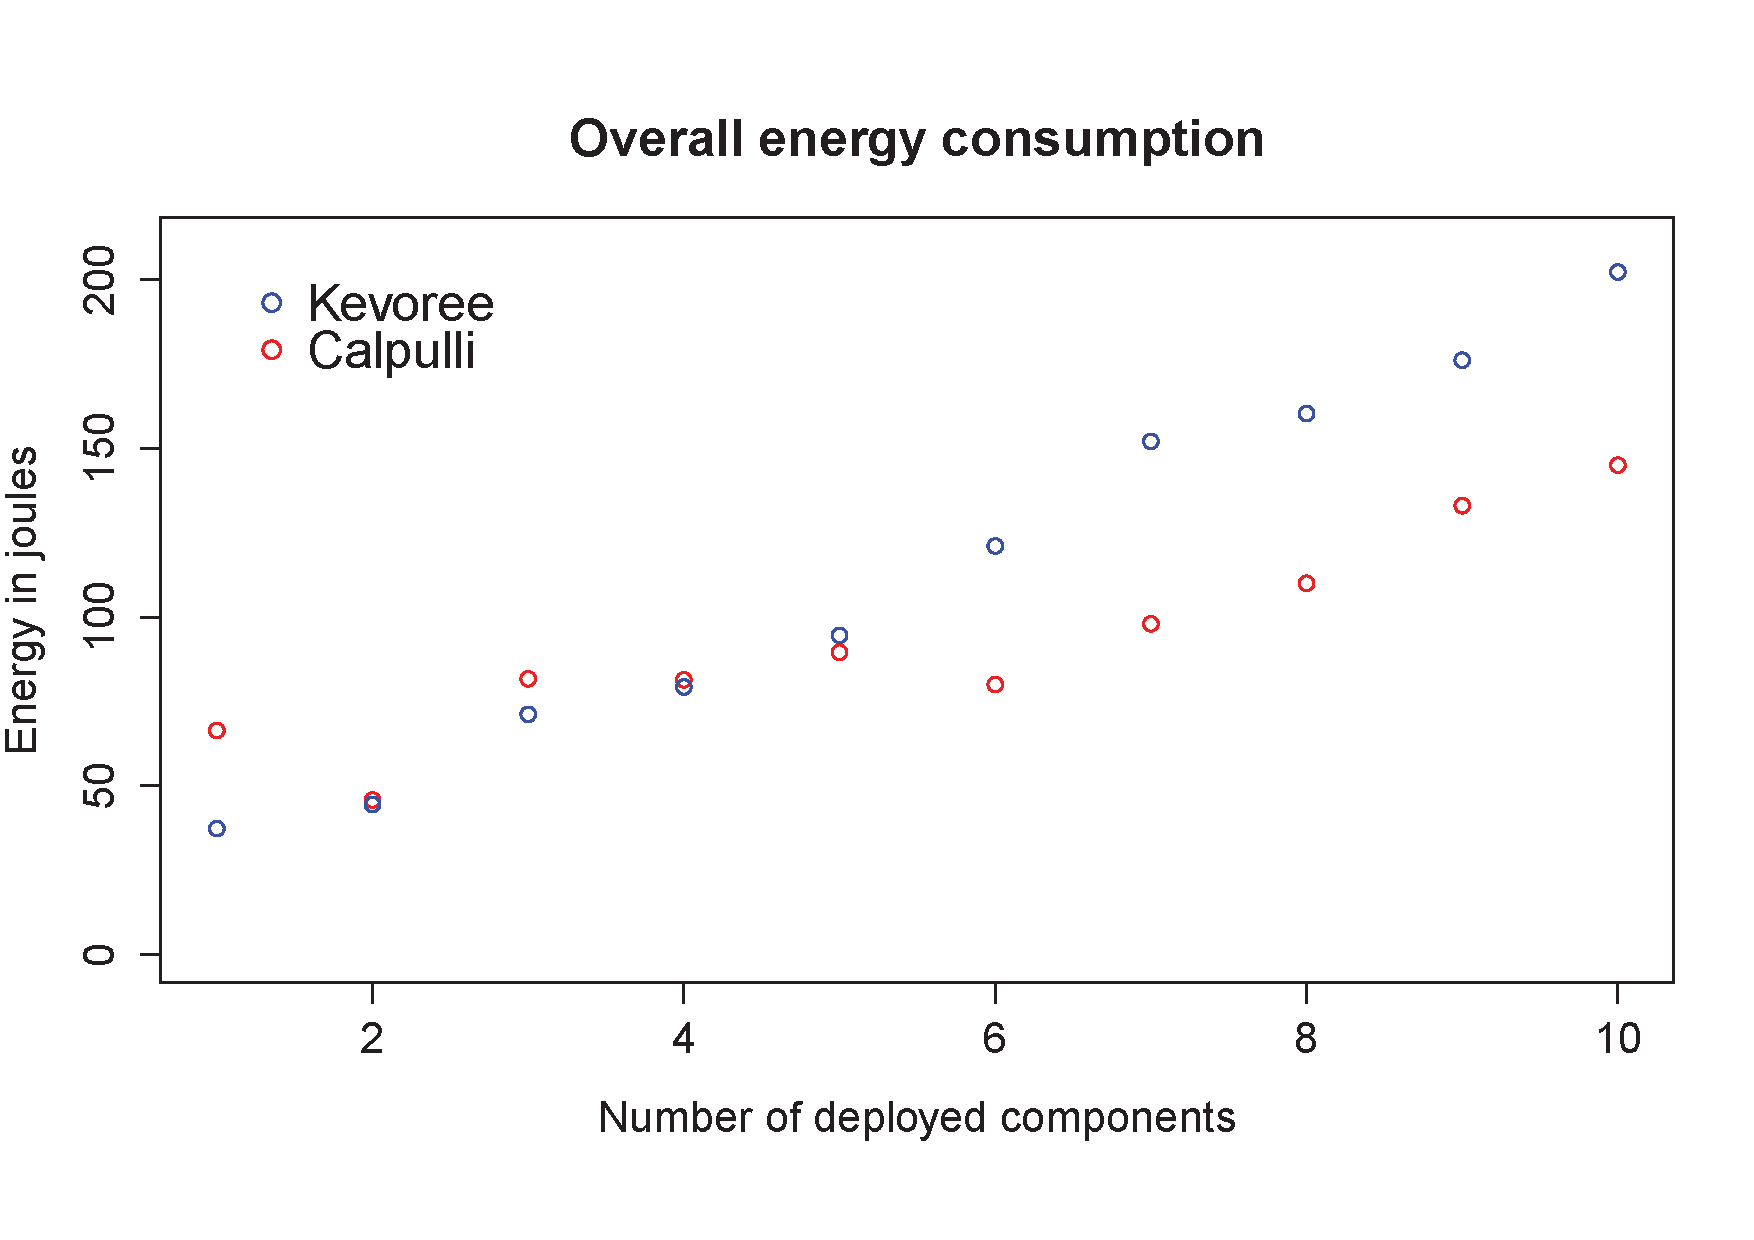
\includegraphics[width=0.95\columnwidth]{chapters/calpulli.images/energyWithFonts.pdf}
	\caption{Energy consumption in the whole network for the given components} \label{fig:Energy}
\end{figure}

The results of these experiments can be observed in Figure \ref{fig:Energy}, where we acknowledge a reduction in the overall consumption when more than 5 components are deployed.

\begin{figure}[htb]
	\centering
	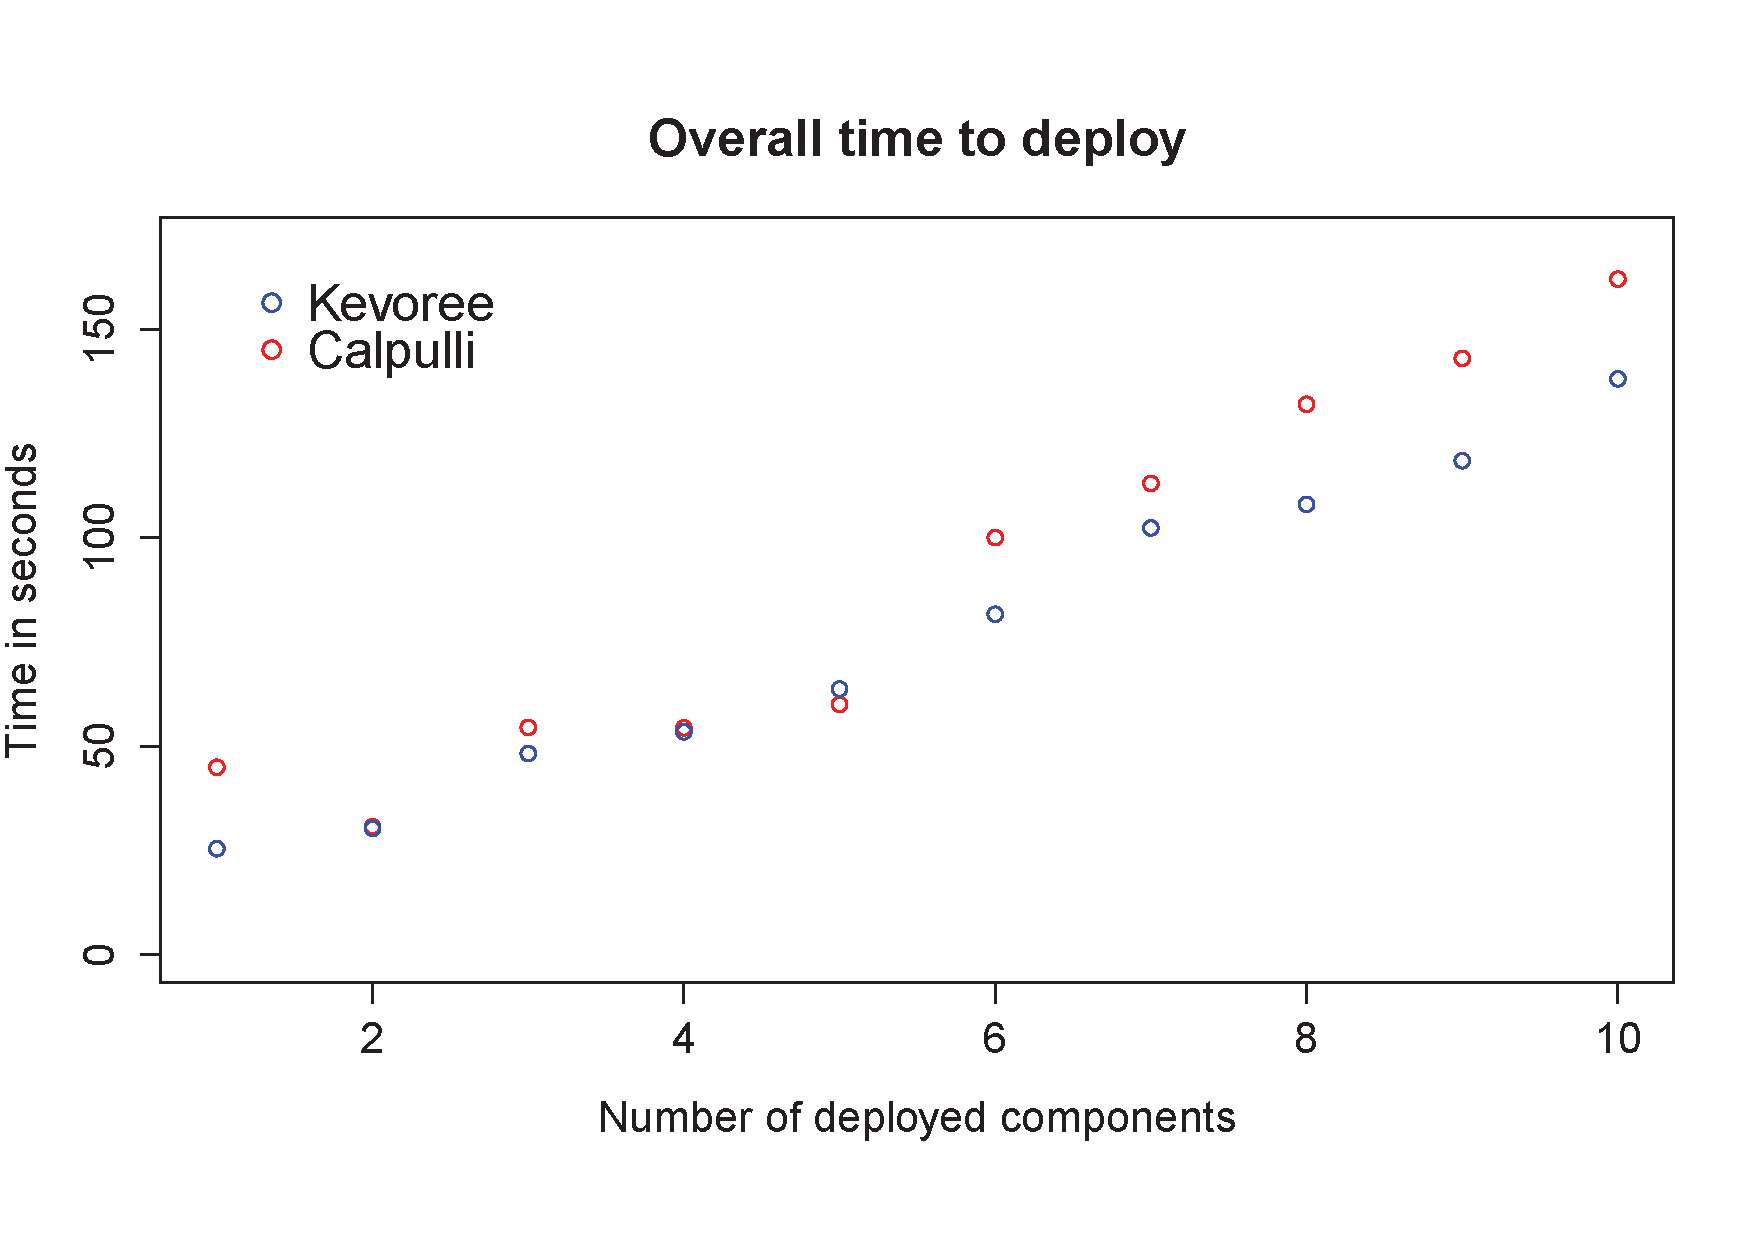
\includegraphics[width=0.95\columnwidth]{chapters/calpulli.images/timeWithFonts.pdf}
	\caption{Time to deploy the selected components} \label{fig:Time}
\end{figure}

\subsection{Evaluation of deployment time}

The time to deploy was also evaluated as a part of a trade-off given by the delay of the analyzed protocols.
In the case of Deluge, as we already state in the previous evaluation, the time to deploy is too high, having only 3 nodes out of 10 working correctly, after the 20 minutes given to the experiment.
For the Kevoree and \textit{Calpulli} algorithms, we can observe in Figure \ref{fig:Time} that the time is approximately the same for 2 and 4 components.
After the fifth component, the time to deploy begins to increase. Since \textit{Calpulli} has a delay in time before downloading the components, caused by the time used to resolve whether it is a repository or not, there is a trade-off between this and the gain in energy consumption. We argue that for larger networks the benefits could be more considerable. We discuss this in our perspectives.

\subsection{Conclusion}
This chapter presented how Kevoree-IoT, our model@runtime implementation, can be used to deal with the problem of software deployment and configuration in Internet of Things systems. 
The main contribution presented is \textit{Calpulli}, a decentralized algorithm which leverages model@runtime information together with the network topology to optimize the distribution of software components, regarding energy consumption and deployment time. 
We highlight that \textit{Calpulli} provides a very good trade-off between deployment time and energy consumption with respect to deluge and the classical Kevoree algorithm.
Indeed, our current Kevoree-IoT implementation along with \textit{Calpulli}, can successfully distribute software components into an IoT network in an efficient manner.

Therefore, two things can be noticed on the execution of our approach:

\begin{enumerate}
	\item We provided a mechanism to distribute software components to specific nodes
	\item and an algorithm to efficiently distribute such components.
\end{enumerate}

With this contributions, we have added adaptation features to nodes being part of an IoT system.
Indeed, each node can perform different types of adaptations and change its behavior regarding the execution state before a new model is disseminated in the network.
Our results show that a trade-off exists on the distribution speed and the energy consumption, resulting in overall energy savings.